\documentclass[12pt, twoside]{scrreprt}
\usepackage[utf8]{inputenc}
\usepackage{amsmath}
\usepackage{parskip}
\usepackage{graphicx}
\usepackage{subcaption}
\usepackage{hyperref}
\usepackage[nameinlink,]{cleveref}
\graphicspath{{./1_Images/}}
\usepackage[a4paper,width=150mm,top=25mm,bottom=25mm]{geometry}
\usepackage{tikz}
\usetikzlibrary{patterns,decorations.pathmorphing,positioning}
%\addtokomafont{disposition}{\rmfamily}

\usepackage{fancyhdr}
\pagestyle{fancy}
\fancyhead{}
\fancyhead[RO, LE]{\rightmark}
\fancyfoot{}
\fancyfoot[RO, LE]{\thepage}
\renewcommand{\headrulewidth}{0.4pt}
\renewcommand{\footrulewidth}{0.4pt}

\usepackage[linesnumbered,ruled,vlined]{algorithm2e}
\usepackage{pythonhighlight}

\usepackage[style=alphabetic,sorting=none]{biblatex}
\addbibresource{references.bib}

\title{
	{Exploration of Time Integration Schemes for Ordinary Differential Equations with Application to Equations of Motion}\\
}

\author{Correa, Alan Jason}
\date{}

\pagenumbering{roman}
\begin{document}

\maketitle

\chapter*{Abstract}
Differential Equations commonly appear in most science and engineering domains. Although analytical solutions to these problems may exist, they are often complicated and can only be determined for fairly simple problems. Furthermore, to model real world engineering problems with sufficient accuracy, differential equations from multiple scientific domains are coupled and solved simultaneously. In such cases, it is almost impossible to analytically solve these differential equations (e.g. Navier-Stokes Equations). However, using numerical techniques, approximate solutions that satisfy the differential equations along with the prescribed boundary and initial conditions could be found. Thus, in the recent past, due to the rise and widespread availability of powerful computing resources, numerical approximations to differential equations have become the preferred way forward.

Numerical time-integration schemes are commonly used for solving initial value problems. Most engineering solver codes already implement these schemes in an efficient manner. However, the aim of this document is to explore and understand time-integration schemes and their algorithms that are already available in literature. Furthermore, a reference implementation of these algorithms in a programming language is sought after. Finally, an attempt is made to apply these algorithms to solve the equations of motion for mechanical systems.




%\chapter*{Dedication}
%hdfjladsfjadhsf

%\chapter*{Declaration}
%dkfhjadfj

%\chapter*{Acknowledgements}
%dfjhasdlf

\tableofcontents

\chapter{Introduction}\label{ch1}
\pagenumbering{arabic}
\section{Initial Value Problems}\label{sec11}
\textit{Initial value problems} are nothing but differential equations that require finding solutions, given the initial conditions at time $t_0$.
\begin{equation}\label{eq101}
\dot{y} = f(t, y) \; with \; y_0 = y(t_0)
\end{equation}
The problem as described in \cref{eq101} is an \textit{ordinary differential equation} of the first order. One can determine the solution analytically using \cref{eq102}.
\begin{equation}\label{eq102}
y(t) = y_0 + \int_{t_0}^{t} f(\tau, y(\tau)) \, d\tau
\end{equation}
In this case, the integral in \cref{eq102} needs to be determined in order to find the solution for time interval of interest. Though it may seem easy, it is often a herculean task to evaluate this integral, particularly when $f(\tau, y(\tau))$ is a non-linear function. 

Furthermore, initial value problems with \textit{higher order} differential equations can be transformed into a system of differential equations and expressed in a vectorized form as shown below.
\begin{equation}\label{eq103}
\begin{gathered}
\dot{\mathit{Y}} = F (t,\mathbf{A}, \mathit{Y}, B) \; with \; \mathit{Y_0} = \mathit{Y}(t_0) \\
\\
\text{where, } 
\mathit{Y} = \begin{pmatrix}
           y_{1}(t) \\
           y_{2}(t) \\
           \vdots \\
           y_{n}(t)
         \end{pmatrix}
\text{, } 
\mathit{\dot{Y}} = \begin{pmatrix}
           \dot{y}_{1}(t) \\
           \dot{y}_{2}(t) \\
           \vdots \\
           \dot{y}_{n}(t)
         \end{pmatrix}
\text{, }
\mathit{Y_0} = \begin{pmatrix}
           y_{1}(t_0) \\
           y_{2}(t_0) \\
           \vdots \\
           y_{n}(t_0)
         \end{pmatrix}
\end{gathered}
\end{equation}

A solution to the formulations as described in \cref{eq103}, where $
\mathbf{A}$ is the System Matrix and $B$ is the Excitation Vector, using a procedure like in \cref{eq102} is complicated often not possible. Hence, it is sought to approximate them numerically using methods that will be discussed hereafter.

\section{Numerical Time Integration Schemes}
\label{sec:timeintegration}
\subsection{Explicit Euler Method}
The Explicit Euler time integration scheme was the first method developed to solve initial value problems. In this scheme, the time derivative $\dot{y}(t)$ in \cref{eq101} is calculated using the \textit{forward difference method}. Therefore, as we march forward in time, the new values of the solution are computed using only known values of the solution at the previous time step \parencite[see][pg. 97]{Fuhrer2001}. 

In short, the Explicit Euler time integration scheme can be summarized as
\begin{equation}
\label{eq104}
y_{n+1} = y_n + h f(t_n, y_n) \text{\hspace{15mm}} n = 0,1,\ldots\\ \\
\end{equation}
where, $y_0 = y(t_0)$ is the initial condition and $h = t_{n+1} - t_n$ is the time increment interval.

The algorithm for procedural implementation of the Explicit Euler time integration scheme is as shown below:
\begin{center}
\smallskip
\begin{minipage}{.7\linewidth}
    \begin{algorithm}[H]
      \SetAlgoLined
      \KwData{$h, n, f(t, y), y_0, t_0$}
      \KwResult{$y_{exp}=\{y_0, y_1, \ldots, y_n\}$ 
      			at $t=\{t_0, t_1, \ldots, t_n\}$ }
      Initialize arrays $y_{exp}=\{y_0\}$ and $t=\{t_0\}$\;
      $y_{i} \gets y_0$ and $t_{i} \gets t_0$\;
      \For{$i \gets 0$ \textbf{to} $n$}  { 
      $y_{i+1} = y_{i} + h f(t_i, y_i)$\;
      $t_{i+1} = t_{i} + h$\;
      Append $y_{exp} \gets y_{i+1}$;
      Append $t \gets t_{i+1}$;
      }
      \Return{$y_{exp}, t$}
     \caption{Explicit Euler Time Integration}
	\label{algo:exp_euler}
    \end{algorithm}
  \end{minipage}
\end{center}

Although this method is fast and can implemented numerically with ease, it is only \textit{conditionally stable} \cite[see][]{Fuhrer2001}. An implementation of the Explicit Euler time integration scheme in python can be found in Appendix A.

\subsection{Implicit Euler Method}\label{sec:implicitEuler}
The Implicit Euler time integration scheme is used to alleviate the stability issues of the Explicit Euler Method. In this scheme, the time derivative $\dot{y}(t)$ in \cref{eq101} is calculated using the \textit{backward difference method}. Therefore, as we march forward in time, the new values of the solution cannot be computed explicitly using known values of the solution at the previous time step \parencite[see][pg. 105]{Fuhrer2001}.
\begin{equation}
\label{eq105}
y_{n+1} = y_n + h f(t_{n+1}, y_{n+1}) \text{\hspace{15mm}} n = 0,1,\ldots\\ 
\end{equation}
where, $y_0 = y(t_0)$ is the initial condition and $h = t_{n+1} - t_n$ is the time increment interval.

It is evident from \cref{eq105} that calculating the solution at the next time step is not straigt forward. However, using the a few mathematical tools that are explined further, the Implicit Euler time integration scheme can be numerically solved.

\subsubsection{Analytical Reformulation}
Given \cref{eq101}, the derivative of the function at every time step can be calculated. Thus, for the time $t_{n+1}$ the we have
\begin{equation}
\dot{y}_{n+1} = f(t_{n+1}, y_{n+1})
\label{eq106}
\end{equation}

Furthermore, \cref{eq105} can be rewritten as 
\begin{equation}
\label{eq107}
y_{n+1} = y_n + h {\dot{y}_{n+1}}
\end{equation}
Now by combining \cref{eq106} and \cref{eq107}, the Implicit Euler time integration scheme can be formulated using only the values of solution ${y_n}$ at previous time step. \parencite[see][]{andasarihandout}
\begin{equation}
\label{eq108}
y_{n+1} = y_n + f(h, t_{n+1}, y_{n}) \\
\end{equation}

As an example of this method, the Implicit Euler time integration scheme for \cref{eq109} can be formulated as shown in \cref{eq110} below.
\begin{equation}
\label{eq109}
\dot{y} = \lambda (y - \sin(t)) + \cos(t)
\end{equation}
\begin{equation}
\label{eq110}
\begin{gathered}
y_{n+1} = y_n + \dfrac{h}{1-h\lambda}f(t_{n+1}, y_{n}) \\
\text{for } n = 0,1,\ldots\\ 
\end{gathered}
\end{equation}

Using the formulation in \cref{eq108}, numerical implementation with time marching is now straightforward. The algorithm for this implementation is as follows:
\begin{center}
\smallskip
\begin{minipage}{.7\linewidth}
    \begin{algorithm}[H]
      \SetAlgoLined
      \KwData{$h, n, f(h, t, y), y_0, t_0$}
      \KwResult{$y_{imp}=\{y_0, y_1, \ldots, y_n\}$ 
      			at $t=\{t_0, t_1, \ldots, t_n\}$ }
      Initialize arrays $y_{imp}=\{y_0\}$ and $t=\{t_0\}$\;
      $y_{i} \gets y_0$ and $t_{i} \gets t_0$\;
      \For{$i \gets 0$ \textbf{to} $n$}  { 
	  $t_{i+1} = t_{i} + h$\;      
      $y_{i+1} = y_{i} + f(h, t_{i+1}, y_i)$\;
      Append $y_{exp} \gets y_{i+1}$;
      Append $t \gets t_{i+1}$;
      }
      \Return{$y_{imp}, t$}
     \caption{Implicit Euler Time Integration - \\%
     using Analytical Reformulation}
	\label{algo:imp_euler_analytical}
    \end{algorithm}
  \end{minipage}
\end{center}

In addition to an easy numerical implementation, this scheme is also \textit{uncondtionally stable}. However, the function $f(h, t, y)$ needs to be found out manually for each problem, thus, limiting its applicability to simple problems and predominantly scalar valued functions $f(t, y)$. 

\subsubsection{Matrix Inversion}
Using \cref{eq109} as an example, \cref{eq107} can be evaluated for $n = 0, 1, 2\ldots$ as
\begin{align}
\label{eq111}
\begin{aligned}
y_{1} &= y_0 + h [\lambda (y_1 - \sin(t_1)) + \cos(t_1)]\\
y_{2} &= y_1 + h [\lambda (y_2 - \sin(t_2)) + \cos(t_2)]\\
\vdots\\
y_{n} &= y_{n-1} + h [\lambda (y_n - \sin(t_n)) + \cos(t_n)]
\end{aligned}
\end{align}
The linear set of equations in \cref{eq111} can be rearranged into \cref{eq112} and then written in matrix form as shown in \cref{eq113}. After inverting the matrix $\mathbf{A}$, we can solve for $\mathbf{y}$ using \cref{eq114}
\begin{align}
\label{eq112}
\begin{aligned}
(1 - h\lambda)y_{1} &= h [\lambda (-\sin(t_1)) + \cos(t_1)] + y_0 \\
(1 - h\lambda)y_{2} - y_1 &= h [\lambda (-\sin(t_2)) + \cos(t_2)]\\ 
\vdots\\
(1 - h\lambda)y_{n} - y_{n-1} &= h [\lambda (-\sin(t_n)) + \cos(t_n)]\\
\end{aligned}
\end{align}
\begin{gather}\label{eq113}
\begin{gathered}[t]
\mathbf{A} \mathbf{y} = \mathbf{b}\\ \\ 
\text{where, } \mathbf{A} = 
\begin{bmatrix}
           (1 - h\lambda) & 0 & \ldots & 0 & 0\\
           -1 & (1 - h\lambda) & \ldots & 0 & 0\\
           \vdots & \vdots & \ddots & \vdots & \vdots\\
           0 & 0 & \ldots & (1 - h\lambda) & 0\\
           0 & 0 & \ldots & -1 & (1 - h\lambda)
\end{bmatrix} \\ \\
\mathbf{y} =
\begin{pmatrix}
           y_{1}\\
           y_{2}\\
           \vdots \\
           y_{n-1}\\
           y_{n}
\end{pmatrix} \text{ and } 
\mathbf{b}=
\begin{pmatrix}
           h [\lambda (-\sin(t_1)) + \cos(t_1)] + y_0\\
           h [\lambda (-\sin(t_2)) + \cos(t_2)]\\
           \vdots \\
           h [\lambda (-\sin(t_{n-1})) + \cos(t_{n-1})]\\
           h [\lambda (-\sin(t_n)) + \cos(t_n)]
\end{pmatrix} 
\end{gathered}
\end{gather}
\begin{equation}
\label{eq114}
\mathbf{y} = \mathbf{A^{-1}} \mathbf{b}
\end{equation}

An algorithm for this implementation is as follows:
\begin{center}
\smallskip
\begin{minipage}{.7\linewidth}
    \begin{algorithm}[H]
      \SetAlgoLined
      \KwData{$h, n, y_0, t_0$}
      \KwResult{$y_{imp}=\{y_0, y_1, \ldots, y_n\}$ 
      			at $t=\{t_0, t_1, \ldots, t_n\}$ }
      Initialize arrays $y_{imp}=\{y_0\}$ and $t=\{t_0\}$\;
	  Initialize vector $\mathbf{b}$ and matrix $\mathbf{A}$\;    
      Setup vector $\mathbf{b}$\; \tcp*[f]{Append $t \gets t_i$ for every row}\; 
      Setup matrix $\mathbf{A}$\;
      Calculate $\mathbf{A^{-1}}$\;
      Calculate $\mathbf{y_{sol}} \gets \mathbf{A^{-1}} \mathbf{b}$\;
      Append $y_{imp} \gets \mathbf{y_{sol}}$\;
      \Return{$y_{imp}, t$}
     \caption{Implicit Euler Time Integration - \\
     using Matrix Inversion}
	\label{algo:imp_euler_matrix}
    \end{algorithm}
  \end{minipage}
\end{center}

Although $\mathbf{A}$ is a sparse matrix, the availability of sophisticated matrix inversion methods for sparse matrices makes the solution of this formulation easily possible. An additional benefit is the elimination of forward time marching. Thus, the solution for the entire time domain is calculated at once. It is, however, important to note that when dealing with initial value problems of higher-order, the size of $\mathbf{A}$ would increase quickly and could lead to problems during matrix inversion. 

\subsubsection{Fixed Point Iteration}\label{sec:implicitEulerIterative}
A fixed point iteration can be applied to solve \cref{eq105}. \parencite[See][pg. 105]{Fuhrer2001}. Thus, we have the following reformulation for the Implicit Euler time integration scheme 
\begin{gather}
\label{eq115}
\begin{gathered}
y^{(j+1)}_{n+1} = y_n + h f(t_{n+1}, y^{(j)}_{n+1}) \\
\text{\hspace{15mm}} j = 0,1,\ldots
\end{gathered}
\end{gather}
In this way, for every step forward in time, we perform additional iterations to converge to a solution. In order to find an initial guess $y^{(0)}_{n+1}$, the Explicit Euler scheme can be used as given in \cref{eq116}. This formulation, thus, comes under the the class of Predictor-Corrector schemes for solving initial value problems.
\begin{equation}
\label{eq116}
y^{(0)}_{n+1} = y_n + h f(t_n, y_n)
\end{equation}
The algorithm for procedural implementation of the Implicit Euler time integration scheme with Fixed Point Iteration is as shown below:
\begin{center}
\smallskip
\begin{minipage}{.7\linewidth}
    \begin{algorithm}[H]
      \SetAlgoLined
      \KwData{$h, n, f(t, y), y_0, t_0, iter_{max}$}
      \KwResult{$y_{imp}=\{y_0, y_1, \ldots, y_n\}$ 
      			at $t=\{t_0, t_1, \ldots, t_n\}$ }
      Initialize arrays $y_{imp}=\{y_0\}$ and $t=\{t_0\}$\;
      Set $convergence \gets True$\; 
      $y_{i} \gets y_0$ and $t_{i} \gets t_0$\;
      \For{$i \gets 0$ \textbf{to} $n$}  {
      	\If{$convergence$} {
		  Initialize $err \gets 1$ and $j \gets 0$\;		  	
		  $y^{j}_{i+1} = y_{i} + h f(t_{i}, y_{i})$\;		  	
		  $t_{i+1} = t_{i} + h$\;
		  \While{$convergence$} {
			$y^{j+1}_{i+1} = y_{i} + h f(t_{i+1}, y^{j}_{i+1})$\;
			$err = abs(y^{j+1}_{i+1} - y^{j}_{i+1})$\;
			$j \gets j+1$\;
			\If(\tcp*[f]{Solution Converged}){$err < tol$}{ 
			  $y_{i+1} = y^{j+1}_{i+1}$\;
    	 	  Append $y_{imp} \gets y_{i+1}$\;
      		  Append $t \gets t_{i+1}$\;
      		  \textbf{break}\;
      		}
      		\If(\tcp*[f]{Solution Diverged}){$j > iter_{max}$}{ 
			  $convergence \gets False$
      		}
      	  }
      	}
      }
      \Return{$y_{imp}, t$}
     \caption{Implicit Euler Time Integration - using Fixed Point Iteration}
	\label{algo:imp_euler_analytical}
    \end{algorithm}
  \end{minipage}
\end{center}
It is important to note that, although this is an Implicit Euler time integration scheme, using fixed point iteration renders this scheme to be \textit{conditionally stable}.

Again, python code implementations for all the Implicit Euler time integration schemes discussed above can be found in Appendix A. 


\subsection{Comparison of Euler Time Integration Schemes}
\begin{figure}[h]
\begin{subfigure}{0.5\textwidth}
\includegraphics[width=\linewidth]{eulercomp1} 
\caption{$\lambda = -4.0, h = 0.5$}
\label{fig:eulercomp1}
\end{subfigure}
\begin{subfigure}{0.5\textwidth}
\includegraphics[width=\linewidth]{eulercomp2}
\caption{$\lambda = -4.0, h = 0.1$}
\label{fig:eulercomp2}
\end{subfigure}
\begin{subfigure}{0.5\textwidth}
\includegraphics[width=\linewidth]{eulercomp3} 
\caption{$\lambda = -10.0, h = 0.2$}
\label{fig:eulercomp3}
\end{subfigure}
\begin{subfigure}{0.5\textwidth}
\includegraphics[width=\linewidth]{eulercomp4}
\caption{$\lambda = -10.0, h = 0.1$}
\label{fig:eulercomp4}
\end{subfigure}
\begin{subfigure}{\textwidth}
\includegraphics[width=\linewidth]{eulercomp5} 
\caption{$\lambda = -4, h = 0.24$}
\label{fig:eulercomp5}
\end{subfigure}
\caption{Solution to $\dot{y} = \lambda (y - \sin(t)) + \cos(t),\; y(0) = 1/\sqrt{2}$}
\label{fig:eulerComparison}
\end{figure}
A graphical representation showing solutions to \cref{eq109} with initial condition $y(0) = 1/\sqrt{2}$, solved with all the above stated time integration schemes with varying parameters $\lambda$ and $h$ can be found in \cref{fig:eulerComparison}. It can be observed that all the three Implicit Euler time integration schemes lead to the same solution. The analytical solution for this initial value problem is given below
\begin{equation}
\label{eq117}
y = (y_0 - \sin t_0)\exp^{\lambda(t-t_0)} + \sin t
\end{equation}


\section{Solution to Example Problems}

// TODO

Solution for $\dot{u} + \gamma u = f$

//TODO

Solution for $\beta \ddot{u} + \alpha \dot{u} + \lambda {u} = f$ - (Only graphs)
Detailed solution will be discussed in next chapter due to similarity with equation of motion


\chapter{Solution Techniques for Equation of Motion}\label{ch2}
\section{Equation of Motion}
The Equation of Motion is one of the most frequently solved equations in engineering and science. It is an outcome of Newton's second law of motion and expresses the equality of internal and external forces for a system.

\begin{figure}[h]
\begin{center}
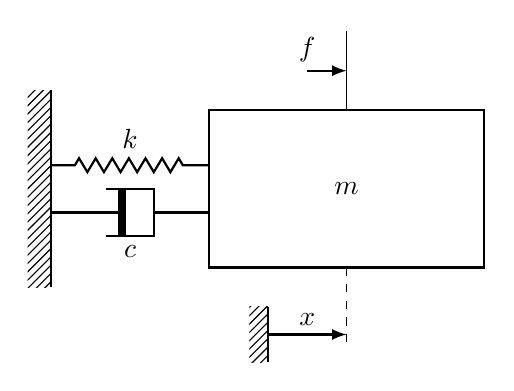
\begin{tikzpicture}[every node/.style={outer sep=0pt},thick,
 mass/.style={draw,thick},
 spring/.style={thick,decorate,decoration={zigzag,pre length=0.3cm,post
 length=0.3cm,segment length=6}},
 ground/.style={fill,pattern=north east lines,draw=none,minimum
 width=0.75cm,minimum height=0.3cm},
 dampic/.pic={\fill[white] (-0.1,-0.3) rectangle (0.3,0.3);
 \draw (-0.3,0.3) -| (0.3,-0.3) -- (-0.3,-0.3);
 \draw[line width=1mm] (-0.1,-0.3) -- (-0.1,0.3);}]

  \node[mass,minimum width=3.5cm,minimum height=2cm,fill=white] (m1) {$m$};

  \node[left=2cm of m1,ground,minimum width=3mm,minimum height=2.5cm] (g1){};
  \draw (g1.north east) -- (g1.south east);

  \draw[spring] ([yshift=3mm]g1.east) coordinate(aux)
   -- (m1.west|-aux) node[midway,above=1mm]{$k$};

  \draw ([yshift=-3mm]g1.east) coordinate(aux')
   -- (m1.west|-aux') pic[midway]{dampic} node[midway,below=3mm]{$c$};

  \foreach \X in {1}  
  {\draw[thin] (m\X.north) -- ++ (0,1) coordinate[midway](aux\X);
   \draw[latex-] (aux\X) -- ++ (-0.5,0) node[above]{$f$}; 
   \draw[thin,dashed] (m\X.south) -- ++ (0,-1) coordinate[pos=0.85](aux'\X);
   \draw[latex-] (aux'\X) -- ++ (-1,0) node[midway,above]{$x$}
    node[left,ground,minimum height=7mm,minimum width=1mm] (g'\X){};
   \draw[thick] (g'\X.north east) -- (g'\X.south east);
  }
  
\end{tikzpicture}
\end{center}
\caption{Simple Oscillatory System}
\label{fig:simpleOscillatorySystem}
\end{figure}
Given a simple oscillatory system as shown in \cref{fig:simpleOscillatorySystem} with a spring having stiffness $k$, a damping element having damping coefficient $c$ and a body having mass $m$ and $x$ as its generalized location co-ordinate, the equation of motion could be written as
\begin{align}
m \ddot{x}(t) + c \dot{x}(t) + k x(t) = f(t) 
\label{eq201}
\end{align}
In \cref{eq201}, the term $m \ddot{x}(t)$ represents the inertia force, $c \dot{x}(t)$ represents the force due to damping element, $k x(t)$ represents the spring force. Together, these terms represent the internal forces and the term $f(t)$ represents the external excitation force on the simple oscillatory system. 

Furthermore, for an oscillatory system with many bodies as shown in \cref{fig:multibodyOscillatorySystem}, a system of equations can be developed and the vectorized equation of motion can be expressed as below
\\ TODO mention non linar form and then linearized form where C = P + G and D = N + K
\begin{equation}
\begin{gathered}
\mathbf{M} \mathit{\ddot{X}}(t) + \mathbf{C} \mathit{\dot{X}}(t) + \mathbf{K} \mathit{X}(t) = \mathit{F}(t) \\
\\
\text{where,}\; 
\mathit{X} = \begin{pmatrix}
           x_{1}(t) \\
           x_{2}(t) \\
           \vdots \\
           x_{n}(t)
         \end{pmatrix}
, 
\mathit{\dot{X}} = \begin{pmatrix}
           \dot{x}_{1}(t) \\
           \dot{x}_{2}(t) \\
           \vdots \\
           \dot{x}_{n}(t)
         \end{pmatrix}
,
\text{and }
\mathit{\ddot{X}} = \begin{pmatrix}
           \ddot{x}_{1}(t) \\
           \ddot{x}_{2}(t) \\
           \vdots \\
           \ddot{x}_{n}(t)
         \end{pmatrix}
\end{gathered}
\label{eq202}
\end{equation}

In \cref{eq202}, $\mathit{X}(t)$ is the vector of generalized location co-ordinates for the system, $\mathbf{M}$ is the Inertia Matrix, $\mathbf{C} \mathit{\dot{X}}(t)$ represents forces due to velocity dependent damping and gyroscopic effects, $\mathbf{K}$ is the Stiffness Matrix and $\mathit{F}(t)$ is the vector of external excitation forces.

\begin{figure}[h]
\begin{center}
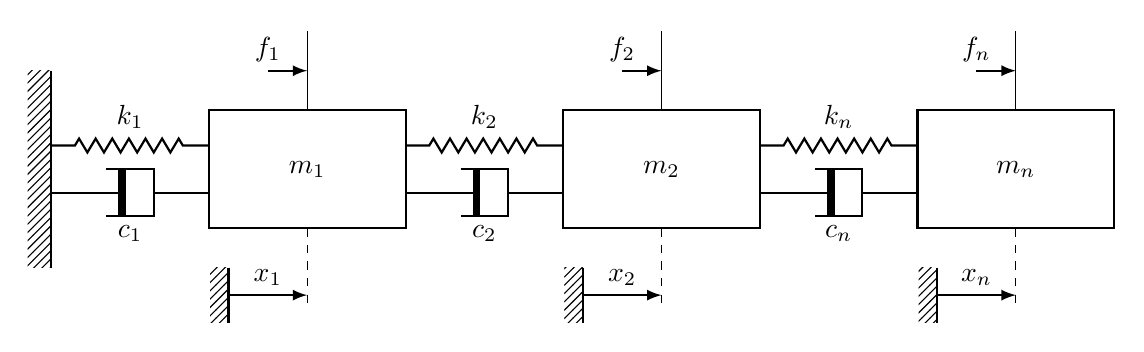
\begin{tikzpicture}[every node/.style={outer sep=0pt},thick,
 mass/.style={draw,thick},
 spring/.style={thick,decorate,decoration={zigzag,pre length=0.3cm,post
 length=0.3cm,segment length=6}},
 ground/.style={fill,pattern=north east lines,draw=none,minimum
 width=0.75cm,minimum height=0.3cm},
 dampic/.pic={\fill[white] (-0.1,-0.3) rectangle (0.3,0.3);
 \draw (-0.3,0.3) -| (0.3,-0.3) -- (-0.3,-0.3);
 \draw[line width=1mm] (-0.1,-0.3) -- (-0.1,0.3);}]

  \node[mass,minimum width=2.5cm,minimum height=1.5cm,fill=white] (m1) {$m_1$};
  \node[mass,minimum width=2.5cm,minimum height=1.5cm,fill=white,right=2cm of
  m1] (m2) {$m_2$};
  \node[mass,minimum width=2.5cm,minimum height=1.5cm,fill=white,right=2cm of
  m2] (mn) {$m_n$};
  
  \node[left=2cm of m1,ground,minimum width=3mm,minimum height=2.5cm] (g1){};
  \draw (g1.north east) -- (g1.south east);

  \draw[spring] ([yshift=3mm]g1.east) coordinate(aux)
   -- (m1.west|-aux) node[midway,above=1mm]{$k_1$};
  \draw[spring]  (m1.east|-aux) -- (m2.west|-aux) node[midway,above=1mm]{$k_2$};
   \draw[spring]  (m2.east|-aux) -- (mn.west|-aux) node[midway,above=1mm]{$k_n$};

  \draw ([yshift=-3mm]g1.east) coordinate(aux')
   -- (m1.west|-aux') pic[midway]{dampic} node[midway,below=3mm]{$c_1$}
     (m1.east|-aux') -- (m2.west|-aux') pic[midway]{dampic} node[midway,below=3mm]{$c_2$}
     (m2.east|-aux') -- (mn.west|-aux') pic[midway]{dampic} node[midway,below=3mm]{$c_n$};

  \foreach \X in {1,2,n}  
  {\draw[thin] (m\X.north) -- ++ (0,1) coordinate[midway](aux\X);
   \draw[latex-] (aux\X) -- ++ (-0.5,0) node[above]{$f_\X$}; 
   \draw[thin,dashed] (m\X.south) -- ++ (0,-1) coordinate[pos=0.85](aux'\X);
   \draw[latex-] (aux'\X) -- ++ (-1,0) node[midway,above]{$x_\X$}
    node[left,ground,minimum height=7mm,minimum width=1mm] (g'\X){};
   \draw[thick] (g'\X.north east) -- (g'\X.south east);
  }
  
\end{tikzpicture}
\end{center}
\caption{Oscillatory System with Many Bodies}
\label{fig:multibodyOscillatorySystem}
\end{figure}

The \cref{eq202} could also represent the equation of motion for a Finite Element Model. In such a formulation, the vector $\mathit{X}(t)$ would then represent the nodal displacements. 

Inorder to solve \cref{eq201} using the Time Integration schemes that were discussed in the previous chapter, it would be helpful to reformulate higher-order differential equation into a set of first-order differential equations. Doing so would eventually lead to the State-Space representation.
\section{State-Space Representation}
Let us define two functions $u(t)$ and $v(t)$ as shown below. On substituting \cref{eq203} in \cref{eq201} we get \cref{eq204}. Further, rearanging \cref{eq204} and rewriting \cref{eq203b} we get a system of first-order ordinary differential equations in \cref{eq205} and \cref{eq206}. Representing these together in a vector formulation gives the \emph{non-linear} form of the State-Space representation. 
\begin{subequations}\label{eq203}
\begin{align}
u(t) &= x(t) \label{eq203a}\\
v(t) &= \dot{x}(t) = \dot{u}(t)\label{eq203b}
\end{align}
\end{subequations}
\begin{align}
m \dot{v}(t) &= -cv(t) - ku(t) + f(t) \label{eq204}\\
\dot{v}(t) &= -\frac{c}{m} v(t) - \frac{k}{m} u(t) + f(t)\label{eq205}\\[3pt]
\dot{u}(t) &= v(t)\label{eq206}\\[10pt]
\begin{pmatrix}
\dot{v}(t) \\[3pt]
\dot{u}(t)
\end{pmatrix}
&= 
\begin{pmatrix}
-\frac{c}{m} v(t) - \frac{k}{m} u(t) + f(t) \\[3pt] 
v(t)
\end{pmatrix}\label{eq207}
\end{align}
In the case of the simple oscillatory system considered, \cref{eq207} turns out to be linear and can be expressed as shown in \cref{eq208}. 
\begin{gather}
\dot{Y}(t)\label{eq208}
= \mathbf{A} Y(t) + B(t) = F(t, \mathbf{A}, Y, B)\\[5pt]
\text{where, } 
\dot{Y}(t) =
\begin{pmatrix}
	\dot{v}(t) \\[3pt]
	\dot{u}(t)
\end{pmatrix}
\text{, }
Y(t) =
\begin{pmatrix}
	v(t) \\[3pt]
	u(t)
\end{pmatrix}
\text{, }
\mathbf{A} =
\begin{bmatrix}
		-\frac{c}{m} & - \frac{k}{m}\\[3pt]
		1 & 0
\end{bmatrix}
\text{and  } 
B(t) =
\begin{pmatrix}
f(t) \\[3pt] 
0
\end{pmatrix}\notag
\end{gather}
Here, \cref{eq208} is called the \emph{linearized} State-Space representation and $\mathit{Y}(t)$ is the \emph{state vector} for the given system of first-order ordinary differential equations. Also, notice that \cref{eq208} is of the form of \cref{eq103} as briefly described in \cref{sec11}. This method can be generalized to any higher-order ordinary differential equation. For eg. one would need define $w(t) = \ddot{x}(t)$ and proceed with the steps as described in \cref{eq203} to \cref{eq207} to finally arrive at the form in \cref{eq208}.

Inorder to proceed with the solution of \cref{eq201}, Initial Conditions need to be provided. Since \cref{eq201} is a second-order differential equation, two initial values are needed. In the case of the simple oscillatory system considered, these would be the initial position $x_0 = x(t_0)$ and initial velocity $v_0 = v(t_0)$. For the vectorized solution schemes, the Initial Condition is prescribed in terms of the state vector at time $t_0$ as shown below.
\begin{equation}\label{eq209}
Y_{0} = Y(t_0) = \begin{pmatrix} v(t_0) \\ u(t_0) \end{pmatrix} = \begin{pmatrix} v_0 \\ u_0 \end{pmatrix}
\end{equation}
\section{Scalar Solution Schemes}
In this section the focus would be to use \cref{eq205} and \cref{eq206} to find a solution to the Equation of Motion by applying the Time Integration schemes as discussed earlier. Although they are simple to implement numerically, scalar solution schemes would lead to lagging of the approximate solution behind the exact solution. This is because while marching forward in time, \cref{eq205} and \cref{eq206} are not simultateously solved.
\subsection{Explicit Euler Method}
On application of the Explicit Euler scheme as described in \cref{eq104} to \cref{eq205} and \cref{eq206}, the following time discretization is obtained for the position $u$ and velocity $v$ of the simple oscillatory system. As it can be seen, marching forward in time is straightforward and only uses values computed in the previous time step. 
\begin{align}
v_{n+1} &= v_{n} + h \; (-\frac{c}{m} v_{n} - \frac{k}{m} u_{n} + f_{n})\label{eq210}\\
u_{n+1} &= u_{n} + h \; (v_{n})\label{eq211}
\end{align}
Due to discretization using the Explicit Euler scheme in \cref{eq211}, for the computation of displacement at next time step $u_{n+1}$, the value of velocity from the previous time step $v_{n}$ is used, eventhough a newer value $v_{n+1}$ is available after computing \cref{eq210}.

//TODO: Add Plot for Solution from Python Code
\subsection{Semi-Implicit Euler Method}
As an improvement to the Explicit Euler scheme, if the newly computed value of velocity at the next time step $v_{n+1}$ is used for the computation of position at the next time step $u_{n+1}$ in \cref{eq213}, the appoximate solution would be improved and the lag of the approximated displacement in comparison to the exact solution would be reduced. 
\begin{align}
v_{n+1} &= v_{n} + h \; (-\frac{c}{m} v_{n} - \frac{k}{m} u_{n} + f_{n})\label{eq212}\\
u_{n+1} &= u_{n} + h \; (v_{n+1})\label{eq213}
\end{align}
It can be seen that \cref{eq213} is the result of application of the Implicit Euler scheme as described in \cref{eq105} to \cref{eq206}, whereas \cref{eq212} is identical to \cref{eq210}, a result of application of Explicit Euler scheme to \cref{eq205}. Hence, this scheme is called Semi-Implicit Euler  Method.

//TODO: Add Plot for Solution from Python Code

\section{Vectorized Solution Schemes}
In this section, solution of the Equation of Motion is sought by using Matrix-Vector methods. Although, their implementation is not as straight-forward as the scalar solution schemes, the phase lag between the approximate solution and the exact solution is eliminated. This results from the simultaneous computation of velocity and position at the next time step by combining them in the \emph{state-vector} as shown in \cref{eq208} and restated below.
\begin{equation}\label{eq214}
 Y(t) =
\begin{pmatrix}
	v(t) \\[3pt]
	u(t)
\end{pmatrix}
 = 
 \begin{pmatrix}
	\dot{x}(t) \\[3pt]
	x(t)
\end{pmatrix}
\end{equation}
\subsection{Explicit Euler Method (Vectorized)}
The vectorized Explicit Euler scheme is obtained by plainly combining \cref{eq210} and \cref{eq211} into \cref{eq215}. Hence, although this is a vectorized solution scheme, the approximate solution for displacement $u(t)$ still lags behind the exact solution. The intial condition $Y_0$ for time stepping is as described in \cref{eq209}.
\begin{gather}\label{eq215}
Y_{n+1} =\; Y_{n} \;+ \; h \; F(t_n, \mathbf{A}, Y_{n}, B_{n})\\[5pt]
\text{where, }
F(t_n, \mathbf{A}, Y_{n}, B_{n})
=
\begin{pmatrix}
-\frac{c}{m} v_{n} - \frac{k}{m} u_{n} + f_{n} \\[3pt] 
v_{n} 
\end{pmatrix}\notag \\
\text{and }
 n = 0, 1, 2, \hdots \notag
\end{gather}

\subsection{Implicit Euler - Iterative Convergence Method}
Building upon Fixed Point Iteration scheme as explained in \cref{sec:implicitEulerIterative} and extending \cref{eq115} and \cref{eq116} to the State-Space representation given by \cref{eq208}, the following Implicit Euler scheme is obtained. Here, \cref{eq216} is the Predictor equation for every new time step and \cref{eq217} is the Corrector equation  that is used for convergence of the approximate solution for the current time step. Although this is an Implicit Euler scheme, numerical approximation errors could lead to divergence when a large time step is used for computations.
\begin{alignat}{3}
\text{Predictor: }& Y_{n+1}^{(j)} &=\; Y_{n} \;+ \;& h \; F(t_n, \mathbf{A}, Y_{n}, B_{n})\label{eq216}\\[0pt]
\text{Corrector: }& Y_{n+1}^{(j+1)} &=\; Y_{n} \;+ \;& h \; F(t_{n+1}, \mathbf{A}, Y_{n+1}^{(j)}, B_{n+1})\label{eq217}
\end{alignat}
\begin{equation}
\text{for } n \text{ and } j= 0, 1, 2, \hdots \notag \\[0pt]
\end{equation}

Another method for obtaining Iterative Convergence is the Newton-Raphson Method where, firstly a Newton Polynomial $G(Y_{n+1}) = 0$ is obtained by applying Implicit Euler scheme to \cref{eq208} as shown below 
\begin{gather}\label{eq218}
Y_{n+1} =\; Y_{n} \;+ \;  \mathbf{A} h Y_{n+1} + h B_{n+1} \notag \\
(\mathbf{I} - \mathbf{A} h) Y_{n+1} + Y_{n} + h B_{n+1} = 0 
\end{gather}
Now, the only unknown in \cref{eq218} is the state-vector at the new time step $Y_{n+1}$. Inorder to find the roots of this Vector Polynomial, the Newton-Raphson Method for vector fields can be utilized. 

//TODO Review and expand Newton-Raphson Method for vector functions

//TODO Add Plot for Solution from Python Code

\subsection{Implicit Euler - Matrix Inversion Method} 
For the Matrix Inversion Method, instead of starting with the state-space representation in \cref{eq208}, the Implicit Euler scheme is applied to \cref{eq205} and \cref{eq206}. As a result, the following two equations are obtained.
\begin{align}
v_{n+1} &= v_{n} + h \; (-\frac{c}{m} v_{n+1} - \frac{k}{m} u_{n+1} + f_{n+1})\label{eq219}\\
u_{n+1} &= u_{n} + h \; (v_{n+1})\label{eq220}
\end{align}
The time discretization expressed in \cref{eq219} and \cref{eq220} is valid for all time steps. By substituing the values for $n = 0, 1,\hdots, n-1$ a linear system of equations \cref{eq221} to \cref{eq226} is developed by keeping known values on the right and unknown values on the left as shown below. 
\begin{alignat}{3}
(1 + h\frac{c}{m})\; &v_{1} +& \;(h\frac{k}{m})u_{1} &= f_{1} + v_{0}\label{eq221}\\
(-h)\; &v_{1} +& u_{1} &= u_{0} \label{eq222}\\
(1 + h\frac{c}{m})\; &v_{2} +& \;(h\frac{k}{m})u_{2} - v_{1} &= f_{2} \label{eq223} \\
(-h)\; &v_{2} +& u_{2} - u_{1} &= 0 \label{eq224}\\
& & &\vdots\notag\\
(1 + h\frac{c}{m})\; &v_{n} +& \;(h\frac{k}{m})u_{n} - v_{n-1} &= f_{n} \label{eq225}\\
(-h)\; &v_{n} +& u_{n} - u_{n-1} &= 0 \label{eq226}
\end{alignat}
This linear system of equations  could then be reformulated as a \emph{matrix-vector} equation as in \cref{eq227}. The solution vector $\mathbf{u}$ to \cref{eq227} is then obtained by \cref{eq228} which requires inverting the matrix $\mathbf{A}$. 
\begin{gather}
\mathbf{A} \mathbf{u} = \mathbf{b}\label{eq227}\\[5pt]
\text{where,}\notag\\ \mathbf{A} = 
\begin{bmatrix}
           (1 + h\frac{c}{m}) & (h\frac{k}{m}) & 0 & 0 & \ldots & 0 & 0 & 0 & 0\\
           (-h) & 1 & 0 & 0 & \ldots & 0 & 0 & 0 & 0\\
           -1 & 0 & (1 + h\frac{c}{m}) & (h\frac{k}{m}) & \ldots & 0 & 0 & 0 & 0\\
           0 & -1 &  (-h) & 1 & \ldots & 0 & 0 & 0 & 0\\
           \vdots & \vdots & \vdots & \vdots & \ddots &\vdots & \vdots&\vdots & \vdots\\           0 & 0 & 0 & 0 &\ldots & (1 + h\frac{c}{m}) & (h\frac{k}{m}) & 0 & 0\\
           0 & 0 & 0 & 0 &\ldots & (-h) & 1 & 0 & 0\\
           0 & 0 & 0 & 0 &\ldots & -1 & 0 & (1 + h\frac{c}{m}) & (h\frac{k}{m})\\
           0 & 0 & 0 & 0 &\ldots & 0 & -1 & (-h) & 1
\end{bmatrix}\notag\\[10pt]
\mathbf{u} =
\begin{pmatrix}
           v_{1}\\
           u_{1}\\
           v_{2}\\
           u_{2}\\
           \vdots \\
           v_{n-1}\\
           u_{n-1}\\
           v_{n}\\
           u_{n}\\
\end{pmatrix} \text{ and } 
\mathbf{b}=
\begin{pmatrix}
          h f_1 + v_0\\
           u_0\\
           h f_2\\
           0 \\
           \vdots \\
           h f_{n-1}\\
           0 \\
           h f_{n}\\
           0 \\
\end{pmatrix} \notag
\end{gather}
\begin{equation}
\\[5pt]
\mathbf{u} = \mathbf{A^{-1}} \mathbf{b} \label{eq228}
\end{equation}

Although, matrix inversion is necessary, using this scheme gives the solution for the complete time interval of the solution at once. %Hence, if a space-time formulation is desired, like in  Structural Mechanics problems, building upon this methodology is key.
 
//TODO Add Plot for Solution from Python Code.

\section{Example Problems - Derivation of Equation of Motion}
\cite[See][]{stutts_daniel_s_1995_4457929}

%\chapter{Conclusion}
%\section{SectionTitle}
Lorem ipsum dolor sit amet, consectetur adipiscing elit. Nulla dapibus dolor a fringilla aliquam. Praesent sed gravida justo, quis tempus metus. Suspendisse a arcu id ex ultrices condimentum. Sed lacinia, purus quis tincidunt rutrum, nibh felis pulvinar urna, convallis auctor quam mi nec neque. Sed consequat tellus eu dui accumsan sodales. Proin eros justo, tincidunt id sagittis a, eleifend vel leo. Praesent interdum arcu est, nec molestie justo pharetra nec. Aliquam ut magna sed purus vehicula facilisis. Aliquam ornare accumsan velit, sed condimentum nibh ornare vitae. Sed non fringilla magna. Suspendisse laoreet lectus justo, et porttitor massa ultricies in. Aliquam venenatis nibh sit amet ipsum facilisis, id aliquam libero tempus.

Phasellus ultrices id metus et luctus. Nullam a enim cursus, sagittis lectus eu, auctor lorem. Nam lacinia tellus lacus, et lacinia justo tempus vitae. Fusce vel tellus massa. Curabitur scelerisque, nisi a vulputate malesuada, nisl ligula finibus sem, commodo ornare ipsum justo vel mi. Aliquam a blandit felis. Nam nec sapien dictum orci suscipit mollis ac a est. Integer non tincidunt elit, a pellentesque magna. Duis dapibus, lorem ac congue lobortis, ante sem sollicitudin purus, vel vehicula justo justo eu massa. Pellentesque tincidunt quam ipsum, quis sollicitudin tellus ultricies eget. Fusce a accumsan ipsum, ut aliquam magna. Cras fringilla est id ipsum pharetra, vel luctus massa ornare.

\subsection{SubsectionTitle}
Nullam luctus tempus enim, nec commodo quam sagittis non. Nunc ornare felis vitae ornare efficitur. Nullam sit amet mi vitae nisi facilisis mollis. In hac habitasse platea dictumst. Quisque vitae accumsan sapien. Morbi elementum vehicula imperdiet. Aliquam facilisis justo a lectus luctus, at finibus lorem faucibus. Etiam nibh elit, aliquet at sodales vel, ultricies eu dolor. Nam hendrerit, sapien vitae tempus pharetra, sem mi laoreet eros, vel porta erat lectus id ex. Suspendisse erat quam, sodales et luctus vel, efficitur eget est. Morbi blandit massa vitae nibh efficitur hendrerit.

Integer tincidunt ligula non posuere molestie. Sed venenatis massa non tellus tincidunt, vitae rutrum massa vehicula. Cras non consequat ante, sed finibus leo. Aenean hendrerit orci et pellentesque bibendum. Orci varius natoque penatibus et magnis dis parturient montes, nascetur ridiculus mus. Sed ultricies, augue vestibulum dictum gravida, nisl mauris molestie arcu, eget condimentum sem lectus nec eros. Pellentesque habitant morbi tristique senectus et netus et malesuada fames ac turpis egestas. Fusce tempor tortor in faucibus tincidunt. Donec condimentum rhoncus ipsum, et tempor sem posuere vitae. Duis pretium purus sed lacus tincidunt, sed rutrum est aliquet.

\subsection{SubsectionTitle}
Donec interdum ullamcorper egestas. Ut blandit purus vitae dui congue, sed placerat justo pharetra. Aenean porttitor neque non lacinia tristique. Phasellus ut purus ultrices velit volutpat tempus. Praesent aliquam dapibus varius. Vivamus sit amet vulputate magna, ac porttitor tortor. Nam ultrices molestie mi sed blandit. Nam posuere massa sapien, a tristique elit gravida sed. Praesent lacus metus, semper et posuere in, venenatis vitae augue. In quis hendrerit magna. 

\appendix
\chapter{Python Code Examples}
\section{Numerical Time Integration Schemes}
The algorithms discussed in section \ref{sec:timeintegration} will work for any given problem. However, for the sake of clarity, the following initial value problem will be used to describe the numerical implementation of the time integration schemes.
\begin{center}
$\dot{y} = \lambda (y - \sin t) + \cos t$
\end{center}

\subsection{Explicit Euler Method}
\begin{python}
def explicit_euler(h, n, f, y_init, t_init):
    # Setting Initial Conditions for the Initial Value Problem
    y_0 = y_init
    t_0 = t_init

    # Initializing Solution Arrays with Initial Values
    y_explicit = np.array(y_0)
    t_explicit = np.array(t_0)

    # Initializing Parameters for Time Integration
    y_next = y_0
    t_next = t_0

    # Marching Forward in Time
    for i in range(n):

        # Calculate Solution at Next Time Step
        y_next = y_next + h * (f(y_next, t_next))

        # Increment Time Step
        t_next = t_next + h

        # Store Values for Plotting
        y_explicit = np.append(y_explicit, y_next)
        t_explicit = np.append(t_explicit, t_next)

    return y_explicit, t_explicit
\end{python}


\subsection{Implicit Euler Method - Analytical Reformulation}
\begin{python}
def f_hty(h, f, t, y):
    # Reformulated Derivative Function in h, t and y
    # Needs to be formulated for the given IVP
    return h * (1 / (1 - h*lmda) * f(y, t))

def implicit_euler_analytical(h, n, f_hty, y_init, t_init):
    # Setting Initial Conditions for the Initial Value Problem
    y_0 = y_init
    t_0 = t_init
	
    # Initializing Solution Arrays
    y_implicit_1 = np.array(y_0)
    t_implicit_1 = np.array(t_0)

    # Initializing Parameters for Time Integration
    y_next = y_0
    t_next = t_0

    # Marching Forward in time
    for i in range(n):

        # Increment Time
        t_next = t_next + h 

        # Calculate Solution at Next Time Step
        y_next = 
         + f_hty(h, f, t_next, y_next)

        # Storing Values for Plotting
        y_implicit_1 = np.append(y_implicit_1, y_next)
        t_implicit_1 = np.append(t_implicit_1, t_next)

    return y_implicit_1, t_implicit_1
\end{python}

\subsection{Implicit Euler Method - Matrix Inversion}
\begin{python}
def implicit_euler_matrix(h, n, y_init, t_init):
    # Setting Initial Conditions for the Initial Value Problem
    y_0 = y_init
    t_0 = t_init

    # Initializing Solution Arrays with Intitial Values
    y_implicit_2 = np.array(y_0)
    t_implicit_2 = np.array(t_0)

    # Initializing Parameters for Solution
    t_next = t_0
    b = np.zeros(n)
    A = np.zeros(n*n).reshape(n, n)

    #Setting Up Vector b
    for i in range(n):
        t_next = t_next + h
        t_implicit_2 = np.append(t_implicit_2, t_next)
        b_n = -h * (lmda * math.sin(t_next) - math.cos(t_next))
        if i==0:
            b[i] = b_n + y_0
        else:
            b[i] = b_n


    # Setting Up Matrix A
    for i in range(n):
        A[i,i] = 1 - h * lmda
        if i > 0:
            A[i, i-1] = -1

    # Matrix Inversion
    A_inv = np.linalg.inv(A)

    # Calculating Solution Space
    # A * y = b -----> y = inv(A) * b
    y_sol = A_inv @ b

    # Adding Initial Value to Solution Space
    y_implicit_2 = np.append(y_implicit_2, y_sol)

    return y_implicit_2, t_implicit_2
\end{python}

\subsection{Implicit Euler Method - Fixed Point Iteration}
\begin{python}
def implicit_euler_iterative(h, n, f, y_init, t_init, maxitr, tol):
	# Setting Initial Conditions for the Initial Value Problem
    y_0 = y_init
    t_0 = t_init
    
    # Initializing Solution Arrays
    y_implicit_3 = np.array(y_0)
    t_implicit_3 = np.array(t_0)

    # Initializing Parameters for Time Integration
    y_next = y_0
    t_next = t_0
    convergence = True

    # Marching Forward in time
    for i in range(n):
        if (convergence):
            # Initialize Error for Convergence testing
            err = 1
            j = 0

            # Predictor - Explicit Euler
            y_next_iter = y_next + h * (f(y_next, t_next))

            # Increment Time
            t_next = t_next + h

            # Iterative Convergence using Corrector
            while(convergence):
                # Store previous iteration to calculate error
                y_prev_iter = y_next_iter

                # Corrector 
                y_next_iter = y_next + h * f(y_next_iter, t_next)


                # Calculate Error
                err = abs(y_next_iter - y_prev_iter)
                
                # Increment Iteration Counter
                j +=1

                # When solution converges 
                if(err < tol):
                    # Use converged Value for next Time Step
                    y_next = y_next_iter

                    # Store Values for Plotting
                    y_implicit_3 = np.append(y_implicit_3, y_next)
                    t_implicit_3 = np.append(t_implicit_3, t_next)
                    break

                # When solution diverges
                if(j > maxitr):
                    convergence = False
                   
    return y_implicit_3, t_implicit_3
\end{python}
\pagebreak[4]

\setcounter{biburllcpenalty}{7000}


\printbibliography
\end{document}